\chapter{Progettazione e codifica}
\label{cap:progettazione-codifica}

\intro{In questo capitolo vengono discusse le scelte progettuali effettuate per poter sviluppare al meglio il lavoro in questione}\\

\section{Tecnologie e strumenti}
\label{sec:tecnologie-strumenti}

Il linguaggio di programmazione scelto per sviluppare il codice necessario a completare gli obiettivi richiesti è stato \textbf{Python} in quanto offre diverse librerie utili per l'apprendimento automatico e il trattamento del linguaggio naturale e utilizzandolo insieme a \textbf{Jupiter Notebook}, un'applicazione che permette di scrivere documenti misti con testo e codice eseguibile, è stato molto più facile realizzare e documentare le analisi sui dati.

\noindent Per poter estrarre il contenuto testuale dai vari documenti è stato scelto di continuare a utilizzare \textbf{Tika-python} che veniva già utilizzato nel primo prototipo fornito dall'azienda, ma per estrarre il testo non strutturato.
Grazie a Tika, è possibile convertire il contenuto del testo in XHTML da diversi formati di file, questo è stato molto utile per poter individuare i vari elementi semantici all'interno dei documenti.
Come scritto precedentemente, però, questa funzione di Tika non opera correttamente con tutti i tipi di formato e non estrae correttamente la struttura delle tabelle.
Per ovviare al problema delle tabelle è stato scelto di utilizzare dei tool di estrazione appositi come \textbf{Pandas}, \textbf{pdfplumber} e \textbf{python-docx} rispettivamente per estrarre tabelle da file HTML, Pdf e Docx.
Questi tool di estrazione appositi, essendo stati creati proprio per questa funzione, restituiscono le tabelle dei documenti con una struttura sicuramente più simile a quella presente nel documento rispetto a come estrarrebbe Tika.
Per portare poi le tabelle ad un livello di astrazione che fosse uguale per tutti i tipi di formato, le tabelle sono state convertite in \emph{DataFrame} di Pandas (struttura dati bidimensionale che può contenere dati di diversi tipi).

Per poter lavorare con l'XHTML fornito da Tika con più semplicità è stato utilizzato \textbf{BeautifulSoup}, una libreria Python che facilita l'estrazione e la manipolazione di dati da questo tipo di file, consente di creare e modificare tag all'interno del codice con il quale si sta lavorando e di estrarre il contenuto presente nei tag stessi.

Il Chat-Completion Model viene preso da \textbf{OpenAI API}, un'API fornita da OpenAI tramite la quale si possono sfruttare i vari modelli offerti per la generazione di testo in linguaggio naturale, mentre il motore di ricerca utilizzato 
è \textbf{Weaviate}, un database vettoriale utile per la ricerca dei dati basata sulla loro semantica e sulle loro relazioni. 

\section{Progettazione e codifica}

\subsection{L'idea}
\label{subsec:ideaProg}
Grazie a Tika riusciamo a convertire il contenuto dei documenti in XHTML in modo tale da poter lavorare con del testo strutturato,
nei documenti dove è già presente una struttura al di sotto, Tika riesce a convertire correttamente il contenuto dei documenti in un XHTML ed è in grado di individuare le intestazioni (e i loro livelli gerarchici h1,h2,...) e tabelle e grazie a questo non è stato difficile riuscire a implementare le funzioni utili per lavorare con i file HTML e Docx.
Per i Pdf, invece, le cose sono state più complesse, gli unici tool individuati che riescono a convertire bene il contenuto dei pdf (come "Aspose") in testo strutturato richiedono una licenza a pagamento e quindi è stato utilizzato comunque Tika.
In questo caso il contenuto viene rappresentato tramite dei tag \emph{div} che rappresentano le singole pagine e ogni riga viene trascritta tramite dei tag \emph{p}. \\

\noindent Qui di seguito vengono descritte le parti di codice sviluppate e le motivazioni per le quali sono state prese determinate scelte.

\subsection{L'architettura}

\label{sec:progettazione-codifica}
La parte di codice sviluppata per questo progetto integra la parte di logica dell'applicazione di un backend già esistente.

\begin{figure}[!h]
    \centering
    \scalebox{0.5}{
        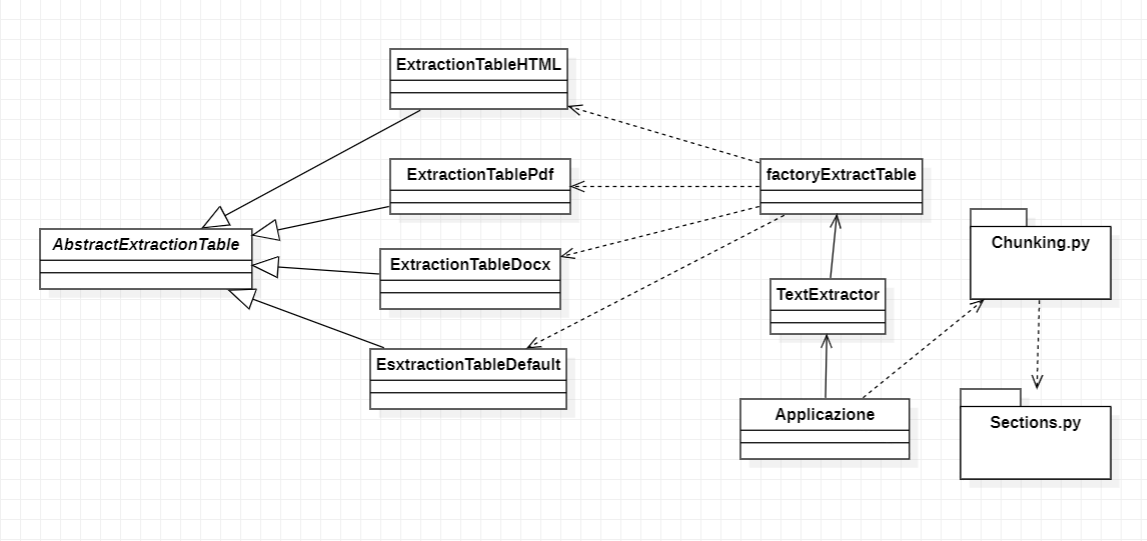
\includegraphics{images/architettura.png}
    }
    \caption{Architettura della parte di codice implementata nel backend.}
\end{figure}

\noindent L'algoritmo prevede come risultato la generazione dei chunk secondo i criteri specificati nel paragrafo \ref{subsubsec:ideachunking}, però, prima di poterli creare c'è bisogno di rielaborare i diversi elementi semantici presi in considerazione.
La classe \textbf{TextExtractor} definisce una funzione \textbf{extractText} che prepara il contenuto del documento alla generazione dei chunk. Inizialmente estrae e converte il testo in XHTML grazie a Tika.
\\\\La parte successiva alla conversione è quella che riguarda l'estrazione delle tabelle dai documenti e la sostituzione di queste ultime linearizzate all'interno del testo che è una parte di algoritmo che varia per i diversi tipi di formato, per questo è stato utilizzato 
il \gls{design pattern}\glsfirstoccur \textbf{\gls{strategy}}\glsfirstoccur: viene definita una classe astratta \textbf{AbstractExtractionTable} che prevede l'implementazione di alcune funzioni come \textbf{ExtractTable} e \textbf{replaceTab}, queste,estraggono la tabella e la sostituiscono con la versione linearizzata all'interno del documento
a seconda del formato preso in considerazione (\textbf{ExtractionTableHTML, ExtractionTableDocx, ExtractionTablePdf}) utilizzando i tool appropriati per l'estrazione delle tabelle come Pandas, python-docx e pdfplumber.
La funzione replaceTab, per i Pdf, funziona in maniera differente rispetto a quella sviluppata per HTML e Docx in quanto, per questi ultimi due formati, le tabelle vengono individuate da Tika, rappresentate dai tag \emph{table} all'interno del testo strutturato e tramite BeautifulSoup sarà facile sostituire il loro contenuto.
Invece, per i Pdf, non vengono utilizzati tag \emph{table} quindi, sono state sfruttate le espressioni regolari per trovare e sostituire le tabelle all'interno del testo grazie a quelle precedentemente estratte e convertite in DataFrame.
Nel caso in cui il formato del file inserito non rientri fra quelli presi in considerazione o non sia ancora stata implementata una classe per quest'ultimo, viene utilizzata la classe \textbf{ExtractionTableDefault}: è stato deciso di implementare questa classe per avere comunque delle possibilità nella sostituizione delle tabelle nel caso in cui si riesca a convertire discretamente il documento in XHTML tramite Tika.
Se vengono trovate poi delle tabelle all'interno del contenuto tramite BeautifulSoup, allora si potranno estrarre tramite Pandas e successivamente sostiure con la linearizzazione.
Per instanziare l'oggetto del tipo ExtractionTable corretto viene utilizzata la funzione \textbf{factoryExtractTable}. 
\\\\Prima di concludere con la funzione extractText bisogna considerare il caso in cui Tika non riesca a convertire correttamente il contenuto in XHTML come spiegato nel paragrafo \ref{subsec:ideaProg}.
Nel caso in cui Tika non riesca a convertire correttamente, quindi non saranno presenti header, viene inserito un tag \emph{h1} che contiene il titolo del file come primo figlio del tag \emph{body}.
Inoltre per semplificare il lavoro che dovrà essere attuato poi in fase di chunking, tutti i tag figli presenti nei \emph{div} che rappresentano le pagine vengono estratti e resi figli del \emph{body}, questo viene fatto in quanto, tramite BeautifulSoup, è più efficiente passare da un tag al suo sibling successivo piuttosto che al tag successivo (che potrebbe essere anche un figlio): al momento dell'estrazione del contenuto se viene estratto il contenuto di un tag \emph{table} verrà estratto tutto il testo presente nella tabella, se passo al tag successivo (che potrebbe essere un \emph{thead}) estrarrò di nuovo il contenuto del figlio avendo così delle informazioni duplicate.
\\\\Al fine di semplificare le operazioni da effettuare sul codice XHTML è stato deciso di creare un modulo Python \textbf{Section.py} che espone la funzione \textbf{makeSection}: questa funzione converte il codice in una struttura ad albero chiamata \emph{Sezione}.
Ogni oggetto Sezione è composto dal titolo del paragrafo (che viene ricavato dagli header presenti nell'XHTML) e dal suo contenuto. Il contenuto è una lista di elementi che può contenere testo o può contenere altre sezioni nel caso in cui ci siano dei sottoparagrafi.
\\\\Infine, grazie alla funzione \textbf{chunking} presente nel modulo \textbf{Chunking.py} viene generata la lista di chunk del documento.
Ogni oggetto Chunk è composto da:
\begin{itemize}
    \item Titolo: titolo del paragrafo al quale corrisponde il suo contenuto;
    \item parentsTit (lista di stringhe): contiene tutti i titoli superiori in senso gerarchico al paragrafo;
    \item contenuto (stringa): porzione di contenuto del paragrafo.
    \item page (intero): numero della pagina da dove è stato preso il contenuto del chunk (ancora non utilizzato, messo per successivi aggiornamenti del codice). 
\end{itemize}

\noindent In questo momento i titoli, i parent dei titoli e il contenuto non venogono ancora concatenati, così, dopo essere entrati in possesso della lista dei Chunk, chi ci lavora può gestirli come preferisce.
L'operazione che viene fatta nel momento della creazione del chunk è la pulizia del testo: la funzione \textbf{cleanText} usa delle espressioni regolari che ricercano sequenze di determinati caratteri uguali e li riduce ad un singolo carattere del tipo individuato, viene chiamata all'interno della funzione chunking.
\\\\
\noindent La parte dell'\textbf{applicazione} effettiva in questo momento è implementata tramite un Jupiter Notebook ed è il prototipo che  è stato reso disponibile all'inizio dello stage dall'azienda.
Sono state aggiunte le chiamate alle funzioni implementate per ottenere le tabelle linearizzate e il chunking migliorato all'interno.
La procedura che viene eseguita per far funzionare il prototipo è la seguente:
\begin{enumerate}
    \item Viene dato un insieme di documenti;
    \item Ogni documento viene convertito in XHTML tramite \textbf{extractText} che a sua volta linearizza le tabelle;
    \item Vengono creati i chunk tramite la funzione \textbf{chunking};
    \item Al contenuto vengono concatenati i titoli dei chunk uniti con i titoli parent tramite la funzione \textbf{createTitleForChunk} da Chunking.py come spiegato nel paragrafo \ref{subsubsec:ideachunking};
    \item I vari chunk vengono caricati sul motore di ricerca;
    \item Quando viene posta una domanda, vengono restituiti i 10 chunk con lo score più alto (hybrid search);
    \item La richiesta (domanda + n chunk, dove n è determinato dalla quantità di token che può prendere in ingresso il Chat-Completion Model) viene consegnata al Chat-Completion Model che elabora le informazioni e restituisce una risposta alla domanda. 
\end{enumerate}


